\section{Management and Orchestration Framework for MEC} \label{framework}

Why need the orchestration and management framework for MEC? gaining tremendous interests...


\subsection{Reference Architecture of MEC}

There are many standard communities such as 3GPP, Open Fog Consortium, and European Telecommunications Standards Institute (ETSI), who are putting their efforts on defining the MEC architectures. 
The reference architecture of MEC, which is initiated by ETSI, is the most popular and well-adopted by both researchers and industries. The ETSI MEC framework is divided into two levels: $i$) Mobile Edge System Level, and $ii$) Mobile Edge Host Level. The former, which provides a global view of complete MEC system, inclues user interface components (i.e, Customer Facing System portal, User App, User App Life-cycle Management Proxy), Operations Support System, and Mobile Edge Orchestration. The latter, which managers the MEC specific functionality of a particular MEC host and the applications running on it, consists of Mobile Edge Manager, Virtualization Infrastructure Manager, and Mobile Edge Host.
%framework standard orchestration framework (ETSI framework)


\begin{figure}[H]
  \begin{center}
   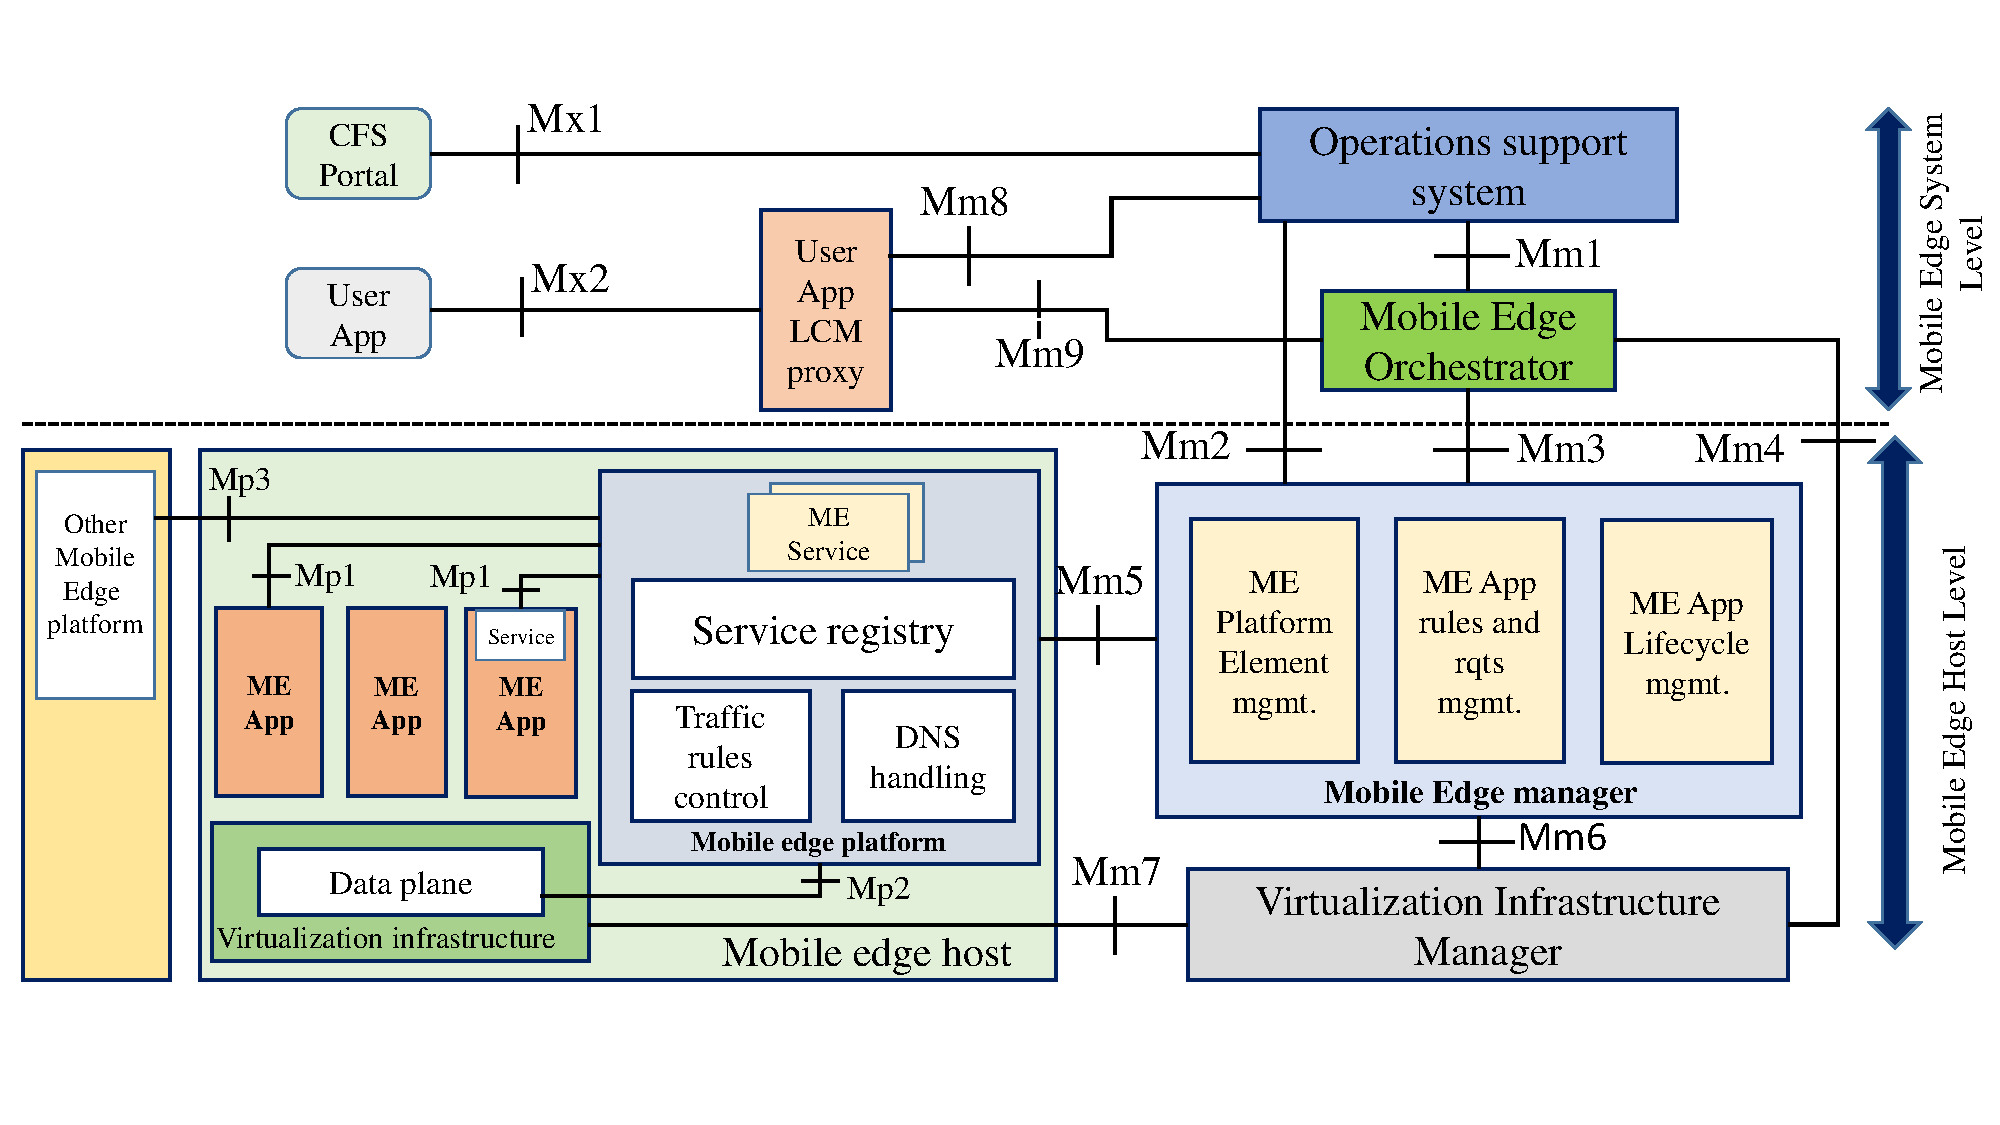
\includegraphics[width=15cm]{./figures/book-etsi-mec.pdf}
   \caption{A reference architecture of MEC}
   \label{fig:etsi-mec}
   \end{center}
\end{figure}


The detailed design of the ETSI MEC framework is presented as follows. 
First, users interact with the ETSI MEC framework through Customer Facing System portal (CFS) and User App. If the users such as tenants are registered and identified, their requests are directly made through the CFS portal. Meanwhile, the ETSI MEC framework also provides an interface to assist various applications, which is called User App. Since the requests from the applications can raise significant security concerns, they are then forwarded to User App Life-cycle Management Proxy before being handled by the framework. To handle the incoming requests, the internal processing components of the MEC frameworks are invoked as follows. First, using standard templates, Operation Support System (OSS) translates the requests to the format, which can be understood by other components. In addition, OSS determines the resource requirements that can be used to serve the requests. Afterwards, the requests are forwarded to Mobile Edge Orchestrator (MEO), which is reponsible for orchestrating the MEC applications across multiple infrastructures. After MEO specifies the infrastructure used to deploy the MEC application, the requests are sent to Mobile Edge Manager (MEM). Since MEM is in charge of the life-cycle management of the applicati  


\subsection{Implementation of the Orchestration and Management Frameworks for MEC}

Real implenmentations such as StarlingX, EdgeX, Akraino,... 
